\section{Описание языка разметки \LaTeX}
\label{sec:latex}
\LaTeX --- система верстки, ориентированная на производство научных математических документов высокого типографского качества. Система также вполне подходит для производства других видов документов, от простых писем до полностью сверстанных книг. \LaTeX использует \TeX в качестве механизма верстки.~\cite{lshort}

К достоинствам выбранного языка разметки можно отнести способ формирования исходного кода, а именно отделение контента от его представления (шаблона, стилевого файла). На первом этапе подготавливается шаблон документа, а затем в ходе выполнения основного приложения в текстовый файл записываются необходимые данные, с соблюдением формата разметки, и запускается компилятор (\texttt{pdflatex}) и на выходе получается готовый .pdf-файл с отчетом о выполненной работе.

К недостаткам данного языка разметки можно отнести большой размер компилятора и сложность построения как стилевых файлов, так и разметки основного документа.

Началом \LaTeX-документа является определение класса документа (например: article, book, report~и~др.)\footnote{в файле отчета использовался сторонний класс extarticle}, который определяет некоторые начальные параметры, такие как уровни, заголовков, поля~и~др. Далее документ разделен на две части: преамбула и основной текст.

В преамбуле определены все параметры документа, переменные, окружения. Также существует возможность вынести все настройки из преамбулы в отдельный файл и подключить его либо как обычный текстовый файл командой \texttt{\textbackslash input\{PATH\}}, либо как стилевой файл \texttt{\textbackslash usepackage\{PATH\}}.

Для выполнения данной работы было создано два стилевых файла: с общими настройками и настройками отображения листингов (эти файлы подробно описаны в разделе~\ref{sec:style}).

Основной текст документа заключен в окружение \texttt{document}.

Структура проекта представлена на рисунке~\ref{fig:tree}. Каталоги \texttt{pics} и \texttt{codes} содержат изображения и листинги соответственно (подробнее, листинги описаны в разделе~\ref{sec:listings}). \texttt{*.sty}-файлы содержат описание стилей. \texttt{main.bib} содержит описание всех использованных в документе ссылок на источники, а \texttt{bibs.tex} --- описание оформления. \texttt{TOC.tex} --- описывает стиль оглавления.

Также отдельно вынесены переменные, используемые в документе, такие как имя студента и преподавателя, название дисциплины~и~др (файл \texttt{info.tex}).

Файл \texttt{solution.tex} формируется автоматически в ходе выполнения основного приложения (листинг~\ref{lst:lab1}).

\begin{figure}[H]
	\centering
	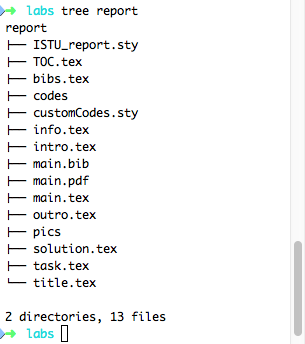
\includegraphics[width=0.5\textwidth]{pics/tree.png}
	\caption{Структура проекта}
	\label{fig:tree}
\end{figure}

Основной текст может содержать в себе следующие элементы:

\begin{itemize*}
	\item простой текст;
	\item заголовки различных уровней;
	\item списки;
	\item листинги;
	\item ссылки, в том числе содержание, алфавитный указатель, список источников, указатель таблиц, формул, иллюстраций~и~др.;
	\item изображения и фигуры\footnote{в данном случае, под фигурами понимаются иллюстрации, сформированными встроенным модулем TikZ или PGF};
	\item таблицы;
	\item формулы;
	\item окружения, определенные пользователем.
\end{itemize*}

Стиль каждого из приведенных элементов может быть настроен отдельно.